The orchestration for this deployment concerns itself with three key areas. The first area, services, 
have been designed utilizing docker containers and docker compose for simple build up and tear down. 
Our docker compose solution utilizes two docker images. The first container utilizes Docker's \hyperlink{https://nginx.org/en/}{NGINX}
image. NGINX was chosen as our webserver for its portability and ease of configuration as a reverse proxy.
Our second container runs a \hyperlink{https://flask.palletsprojects.com/en/3.0.x/}{flask} server. 
The flask server allows us to run web services locally, which are then accessed by NGINX to serve to clients.

The second area, defense, utilizes \hyperlink{https://opencanary.readthedocs.io/en/latest/}{OpenCanary} 
and \hyperlink{https://www.redhat.com/sysadmin/iptables}{iptables}. OpenCanary serves as a honeypot, a target 
designed to waste the time and enumerate the techniques utilized by would-be aggressors. The command-line program, 
iptables, is a series of rules and conditions used to control traffic control into and out of a machine. OpenCanary 
is deployed as a docker container, though the complexity in building it warrants its own separate orchestration. To accomplish this, we utilize some basic bash scripting to automate the necessary commands to run OpenCanary with the configuration and 
services required. To supplement this, we issue some iptables commands as part of this bash script. These rules filter ports and 
drop traffic that attempts to enumerate OpenCanary and its ports. 

Our final area of focus is automation. By automating the setup of our deployment, our services and defenses can be deployed quickly and by a greater number of individuals, even those not intimately familiar with its inner workings. 
The use of docker containers and docker compose also allow our deployment to be mobile, only requiring 
prospective users to install a small number of programs (i.e., docker, docker compose, git). We further simplify this 
setup for users by automating the installation of these programs from within a bash script.

The host server has 4 docker containers running on it. These are Flasky, Fnginx, SQL, and Opencanary. Fnginx acts a proxy for the Flasky container, which is what hosts everything and reaches out to the weather api endpoints. Opencanary doesn't directly interact with any of these functions, but remains functional as a separate container to distract attackers by having multiple open ports.

\begin{figure}[h]
    \centering
    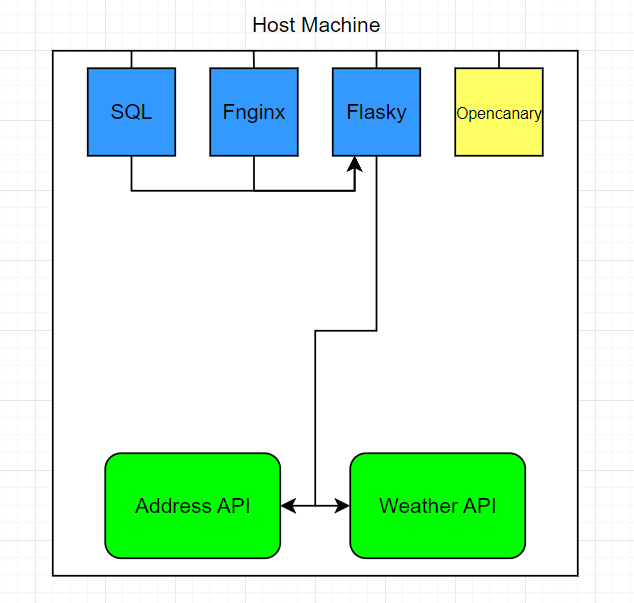
\includegraphics[width=.8\linewidth]{Orch_Diagram.png}
    \caption{A diagram representing the orchestration of the deployment, with API endpoints (green), docker containers offering services (blue), and a honeypot (yellow).}
    \label{fig:enter-label}
\end{figure}
